\chapter{Visione artificiale}

La visione artificiale è un campo che include i metodi per l'acquisizione, elaborazione,analisi e comprensione delle immagini,ed in generale , dati ad alta dimensionali acquisiti dall'ambiente circostante per produrre informazioni numeriche o simboliche, ad esempio, sotto forma di decisioni. Un tema chiave nello sviluppo di questo campo è replicare le capacità di visione umana, la percezione e comprensione di un'immagine con ausili informatici. Questa comprensione dell'immagine può essere vista come la separazione delle informazioni simboliche dai dati di immagine utilizzando modelli costruiti con l'aiuto di geometria, fisica, statistica e teoria dell'apprendimento. La visione artificiale rappresenta anche un campo avente vaste applicazioni industriali per il controllo di processo, tracciabilità, sicurezza, calibrazione.

I dati immagine possono assumere molte forme, come ad esempio sequenze video, viste della stessa scena da più telecamere, o dati multidimensionali da uno scanner medico . Come disciplina tecnologica , la visione artificiale cerca di applicare le sue teorie e modelli realizzare sistemi in grado di ``capire'' ed estrarre le informazioni.

Sottodomini di computer vision includono la ricostruzione delle scene, il rilevamento degli eventi, il monitoraggio video, riconoscimento di oggetti, l'apprendimento, l'indicizzazione, la stima del movimento  e il ripristino dell'immagine .

\section{Processamento delle immagini}

La moderna tecnologia digitale ha reso possibile manipolare 
segnali multidimensionale con sistemi che vanno da semplici circuiti digitali a elaboratori paralleli avanzati

\subsection{Immagine reale} 
Un'immagine definita nel "mondo reale" è considerata una funzione di due variabili reali,
per esempio, $a(x, y)$ dove a rappresenta la luminosità dell'immagine nella cordinata (x,y) 
coppia reale. Un immagine a sua volta può essere considerata contenere sotto-immagini definite
regioni di interesse, ROI o semplicemente regioni.
Questo concetto riflette il fatto che le immagini contengono spesso collezioni di oggetti ciascuno dei quali può essere la base per una
regione.
In un sistema di elaborazione dell'immagine dovrebbe essere possibile applicare
specifiche operazioni di elaborazione delle immagini per le regioni selezionate. 
Le ampiezze di una data immagine saranno quasi sempre essere numeri reali o
numeri interi. Quest'ultimo è di solito un risultato di un processo di quantizzazione che
converte un intervallo continuo (per esempio, tra 0 e 100\% in per un numero discreto di
livelli. In alcuni processi di formazione dell'immagine, tuttavia, il segnale può derivare dal
conteggio di fotoni che implica un intrinseca natura quantizzata.
In altre procedure di formazione dell'immagine, come la risonanza magnetica, la
misura fisica diretta produce un numero complesso in forma di un vero
ampiezza e fase reale.

\subsection{Immagine digitale}

Un'immagine digitale $a[m, n]$ descritta in uno spazio discreto 2D è derivata da un ingresso analogico
a(x, y) in uno spazio continuo 2D attraverso un processo di campionamento che è
spesso indicato come la digitalizzazione.
L'immagine 2D continua $a(x, y)$ è divisa in N righe ed M colonne. l'intersezione di una riga ed una colonna è definita pixel. Il valore assegnato alle coordinate intere $[m, n]$ con ${m = 0,1,2, ..., M-1}$ e ${n = 0,1,2, ..., N-1}$ è
$a[m, n]$. 
Nella maggior parte dei casi il segnale  $a(x, y)$ - che potremmo considerare il segnale fisico
che incide sulla faccia di un sensore 2D - è in realtà una funzione di molte
variabili tra cui profondità $(z)$, colore $(\lambda)$, e tempo $(t)$.
Se non diversamente indicato, si prenderà in considerazione il caso  2D, monocromatico, e con immagini statiche.



L'immagine digitale è la rappresentazione numerica di una immagine
bidimensionale. La rappresentazione può essere di tipo vettoriale oppure
raster (altrimenti detta bitmap); nel primo caso sono descritti degli elementi
primitivi, quali linee o poligoni, che vanno a comporre l'immagine; nel
secondo l'immagine è composta da una matrice di punti, detti pixel, la cui
colorazione è definita (codificata) tramite uno o più valori numerici (bit).

\subsubsection{Immagine bitmap}

In questo tipo di immagini, i valori memorizzati indicano le caratteristiche
di ogni punto dell'immagine da rappresentare (pixel): nelle immagini a colori,
viene memorizzato solitamente il livello di intensità dei colori fondamentali
(nel modello di colore RGB, uno dei più usati, sono tre: rosso, verde e blu.
Un altro esempio è CMYK, usato per la stampa, basato su quattro colori
fondamentali: ciano, magenta, giallo e nero.) nelle immagini monocromatiche in
scala di grigio (dette impropriamente bianco e nero) il valore indica
l'intensità del grigio, che varia dal nero al bianco. Il numero (detto anche
``profondità'') di colori o di livelli di grigio possibili dipende dal massimo
numero di combinazioni permesse dalla quantità di bit utilizzata per ognuno di
questi dati: un'immagine con 1 bit per pixel avrà al massimo due combinazioni
possibili (0 e 1) e quindi potrà rappresentare solo due colori o solo bianco e
nero; nelle immagini a 4 bit per pixel, si possono rappresentare al massimo 16
colori o 16 livelli di grigio; un'immagine a 8 bit per pixel, 256 e così via.
Oltre a questi dati, è solitamente presente un header, che contiene diverse
informazioni sull'immagine, a partire dal numero di righe e colonne di pixel:
le dimensioni sono necessarie per poter dividere e disporre la sequenza di
pixel in linee, in modo da formare una griglia rettangolare di punti, simile
ad un mosaico, in cui ogni riga è formata da un numero preciso (indicato
appunto dal valore larghezza) di tessere. La tecnica utilizzata per queste
immagini, rappresentate da una matrice NxM, dove N è il numero delle righe di
pixel dell'immagine e M delle colonne, è detta raster. Le immagini bitmap
possono essere memorizzate in diversi formati, spesso basati su un algoritmo
di compressione, che può essere lossy (in cui c'è perdita di informazione),
come nelle immagini JPEG, oppure lossless (senza perdita), come nel caso dei
file d'immagine GIF o PNG. Questo tipo di immagini può essere generato da una
grande varietà di dispositivi d'acquisizione: scanner e fotocamere digitali
(contenenti dei sensori CCD o CMOS), ma anche da radar e microscopi
elettronici; inoltre possono venire sintetizzate anche a partire da dati
arbitrari, come funzioni matematiche bidimensionali o modelli geometrici
tridimensionali.


\begin{figure}
\centering
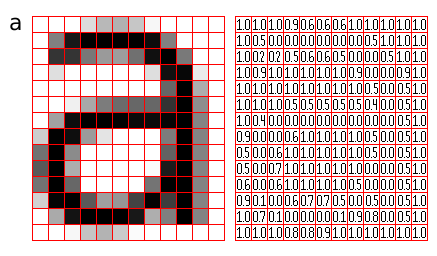
\includegraphics[width=.5\textwidth]{img/image-grid.png}
\caption{Rappresentazione numerica di un immagine}\label{fig:image-grid}
\end{figure}

\subsection{Tipi di operazioni sulle immagini}
I tipi di operazioni che possono essere applicati all'immagine digitale $a[n,m]$
per trasformarla nell'immagine $b[n,m]$ possono essere classificate in 3 categorie

\begin{description}
\item[Puntuali:] 	L'uscita di un operazione a delle determinate coordinate dipende solo dal valore di input a quelle coordinate.
\item[Locali: ] L'uscita di un operazione a delle determinate coordinate dipende dai valori di ingresso in un ``vicinato'' (neighborhood) delle stesse coordinate.
\item[Globali: ] L'uscita di un operazione a delle determinate coordinate dipende dai valori di ingresso di tutta l'immagine.
\end{description}


\begin{figure}
\centering
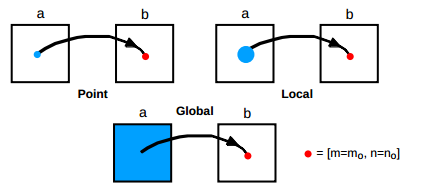
\includegraphics[width=.5\textwidth]{img/puntuale-locale-globale.png}
\caption{Operazione puntuale, locale,globale.}\label{fig:puntuale-locale-globale}
\end{figure}

\subsection{Istogramma dei livelli di grigio}

Per ogni livello di grigio, riporta il numero di pixel 
aventi quel valore,esso è utile per comprendere in maniera 
immediata le caratteristiche dell’immagine e 
individuare eventuali modifiche che possano 
migliorare la sua qualità.
\begin{figure}
\centering
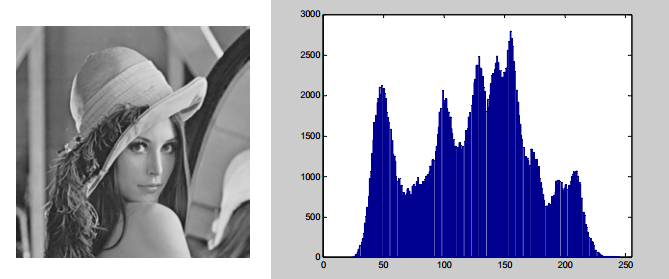
\includegraphics[width=.5\textwidth]{img/histogramma.png}
\caption{Istogramma dei livelli di grigio.}\label{fig:istogramma}
\end{figure}
\`{E} possibile applicare degli operatori puntuali basati sull'istogramma sotto forma di un opportuna trasformazione, tali trasformazioni sono tipicamente orientate al miglioramento della qualità dell’immagine (image
enhancement), esse si realizzano generalmente tramite una funzione 
y=y(x), che ad un livello di grigio x dell’immagine in 
ingresso, fa corrispondere il valore y per l’immagine 
in uscita. La trasformazione si può realizzare anche tramite delle 
Look-up Table (LUT) che permettono 
un’implementazione hardware efficiente.
Le operazioni principali applicabili sono
\begin{itemize}
\item Inversione dei livelli di grigio
\item Compressione logaritmica
\item Compressione potenza
\end{itemize}
\begin{figure}[h]
\centering
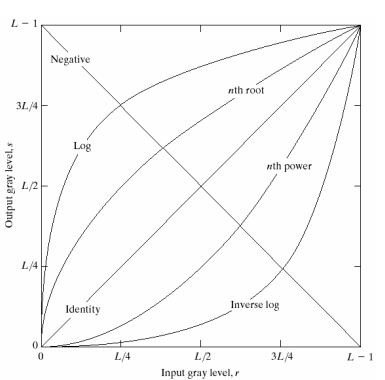
\includegraphics[width=.5\textwidth]{img/trasformazione-istogramma.png}
\caption{Trasformazioni su istogramma.}\label{fig:trasformazione-istogramma}
\end{figure}
\begin{figure}[h]
\centering
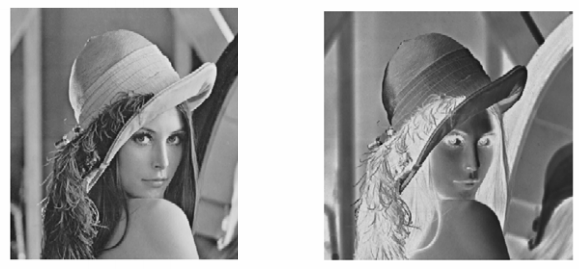
\includegraphics[width=.5\textwidth]{img/inversione-grigio.png}
\caption{Inversione dei livelli di grigio.}\label{fig:inversione-grigio}
\end{figure}
\begin{figure}[h]
\centering
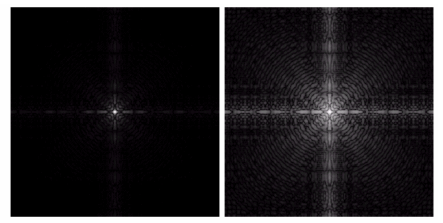
\includegraphics[width=.5\textwidth]{img/compressione-logaritmica.png}
\caption{Compressione logaritmica.}\label{fig:compressione-logaritmica}
\end{figure}
\begin{figure}[h]
\centering
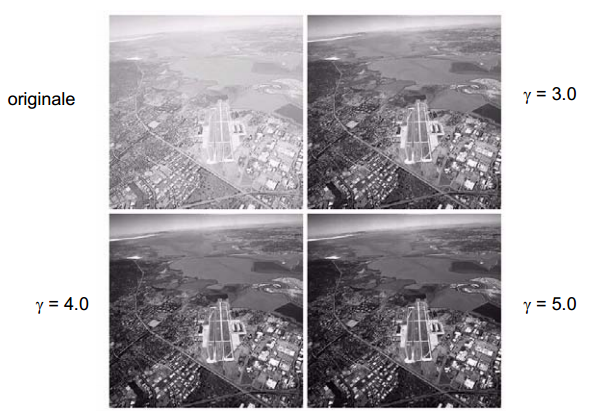
\includegraphics[width=.5\textwidth]{img/compressione-potenza.png}
\caption{Compressione potenza.}\label{fig:compressione-potenza}
\end{figure}

\subsubsection{Espansione del contrasto}
L'espansione del contrasto si realizza per aumentare la dinamica di 
un’immagine il cui istogramma è concentrato 
in un intervallo limitato dei valori possibili,
consideriamo ad esempio una trasformazione del tipo:
\[
y(x) =
  \begin{cases}
   0       & \text{se } x < 150 \\
   \frac{255  (X-150)}{150}       & \text{se } x \geq 150
  \end{cases}
\]

essa è in grado di rimappare la gamma dinamica nell'intervallo visibile in figura \ref{fig:espansione-contrasto}

\begin{figure}
\centering
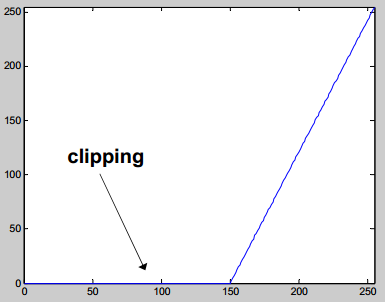
\includegraphics[width=.5\textwidth]{img/espansione-contrasto.png}
\caption{Esempio di espansione del contrasto.}\label{fig:espansione-contrasto}
\end{figure}

\subsubsection{Equalizzazione dell'istogramma}
E’ una tecnica che mira a modificare la forma 
dell’istogramma redistribuendo i valori dei 
livelli di grigio in modo che l’istogramma sia 
quanto più uniforme possibile con l’obiettivo  di migliorare l’immagine a 
debole contrasto, tuttavia, un’equalizzazione non porta 
necessariamente ad un miglioramento dell’immagine (Es. immagine con istogramma 
bimodale).
\begin{figure}
\centering
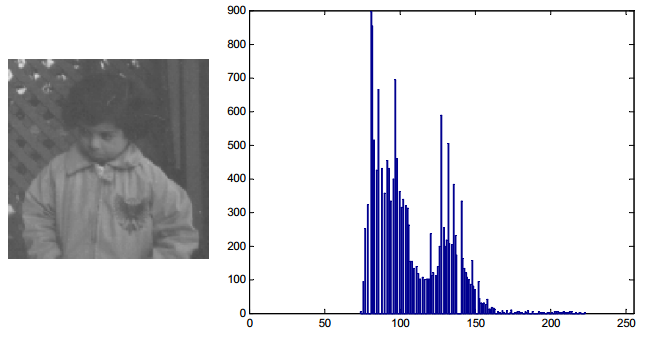
\includegraphics[width=.5\textwidth]{img/equalizzazione-prima.png}
\caption{Prima dell'equalizzazione.}
\label{fig:equalizzazione-prima}
\end{figure}

\begin{figure}
\centering
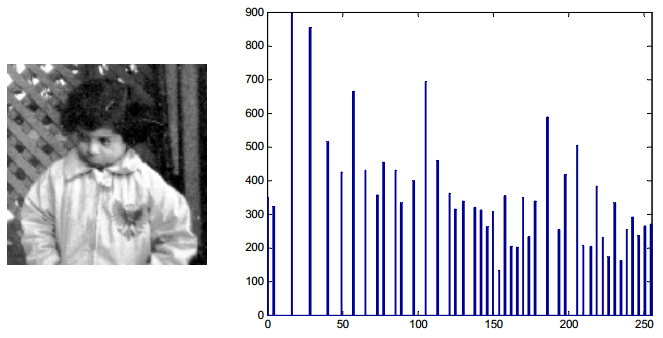
\includegraphics[width=.5\textwidth]{img/equalizzazione-dopo.png}
\caption{Dopo l'equalizzazione.}
\label{fig:equalizzazione-dopo.}
\end{figure}

\subsection{Binarizzazione} In molti casi gli le scene di interesse conducono
ad immagini che possono essere  considerate binarie, cioè contenenti nel caso
ideale solo due livelli di grigio (bianco, nero) ad esempio : testo stampato,
manoscritto, parti meccaniche piatte, sagome, in altri casi, le immagini in
analisi sono  intrinsecamente a più livelli di grigio, ma  l’unico contenuto
rilevante è dato dalla forma  degli oggetti, delle regioni o delle linee.
Anche in queste circostanze il modello ideale  è un’immagine a due livelli.
Dopo l’acquisizione di una scena da parte di un dispositivo di imaging,
l’immagine che si ottiene è comunque  formata da numerosi livelli di grigio
(tipicamente 256).Le ragioni sono principalmente riconducibili  a
illuminazione non omogenea della scena,banda limitata del sistema che limita
la ripidezza  dei fronti in corrispondenza dei bordi e distorsioni impresse
dal sistema ottico. Sono quindi necessari degli algoritmi per la
trasformazione di un’immagine a livelli di  grigio in immagine binaria
(binarizzazione), in  modo da conservare quanto più possibile il  contenuto
rilevante. In letteratura sono stati proposti numerosi  algoritmi di
binarizzazione, ciò è giustificato  dall’intrinseca difficoltà del problema e
dalla  diversità delle caratteristiche delle immagini  da trattare.


\subsubsection{Soglia fissa}

La soluzione più semplice è quella di fare uso 
di una soglia fissa S per cui la binarizzazione 
si realizza tramite la trasformazione.

\[
a(x,y) =
  \begin{cases}
   0       & \text{se } x < S \\
   1       & \text{se } x \geq S
  \end{cases}
\]

La difficoltà in questo caso è data  dall’individuazione del valore della
soglia $S$  che renda efficace l’operazione di  binarizzazione. Esistono
diversi metodi per valutare la soglia  automaticamente a partire
dall’istogramma  dei livelli di grigio dell’immagine originale.

\subsection{Soglia basata su istogramma}

In alcuni casi favorevoli, l’istogramma  dell’immagine da binarizzare presenta
un  andamento nettamente bimodale, sono cioè presenti due picchi (modes) che
rappresentano distintamente lo sfondo e gli  oggetti presenti nella scena, in
questo caso, la soglia viene fissata in  corrispondenza del punto di minimo
tra i due  picchi,la determinazione della soglia richiede quindi  la
preventiva individuazione dei due picchi  nell’istogramma. Mentre
l’individuazione del primo dei due  picchi è semplice (coincide con il livello
di  grigio a massimo valore nell’istogramma),  trovare il secondo picco può
essere più  difficile, in quanto non è detto che coincida  con il secondo
valore più grande  nell’istogramma.

\subsection{Compensazione dello sfondo}

Al segnale d’immagine può spesso  sovrapporsi un segnale spurio di fondo che
si  produce nel corso dell’acquisizione  dell’immagine e dovuto
all’illuminazione della  scena o alla disomogeneità del fondo, e’ opportuno
rimuovere tale segnale spurio  (compensazione dello sfondo) prima della
binarizzazione in quanto potrebbe causare  degli artefatti nell’immagine
binarizzata.

La compensazione dello sfondo può essere  semplicemente realizzata
sottraendo  dall’immagine da trattare l’immagine dello  sfondo ripreso in
assenza di oggetti e  mantenendo le stesse condizioni di  illuminazione e di
configurazione del sensore. Se l’immagine dello sfondo “vuoto” non è
disponibile, si può utilizzare in sua vece il  risultato di un filtraggio
dell’immagine  ottenuto con un filtro di media molto ampio.

\subsection{Operatori locali}
Questi operatori sono usati per miglioramento della qualità di un’immagine (come per gli 
operatori puntuali) e per l' estrazione di caratteristiche dell’immagine (immagine in 
ingresso $\to$ immagine delle caratteristiche).
Il valore di uscita dell’operatore nel punto (i,j) 
dipende solo dai valori di ingresso in un vicinato del 
punto (i,j), vicinato che di solito viene definito in maniera simmetrica 
rispetto al punto (i,j), tali operatori possono essere di tipo lineare o non lineare.

Nei filtri lineari l’uscita è una combinazione lineare dei valori dei 
pixel di ingresso, i coefficienti della combinazione sono disposti su una 
sottoimmagine delle stesse dimensioni del vicinato del punto, in
modo da corrispondere ai punti che vanno a pesare.
La sottoimmagine viene definita maschera o filtro (filter, mask, 
kernel). Perciò si parla di filtraggio spaziale.La valutazione di un 
operatore locale richiede che la maschera sia applicata su tutti i punti 
dell’immagine, tale processo corrisponde alla convoluzione. 

\begin{figure}
\centering
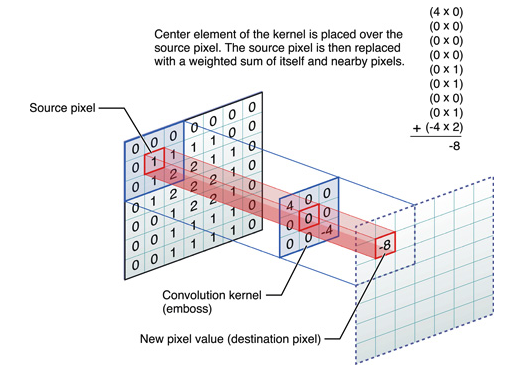
\includegraphics[width=.8\textwidth]{img/convoluzione.png}
\caption{Applicazione di un operatore locale.}
\label{fig:convoluzione}
\end{figure}

\subsection{Filtri di smoothing}

I filtri di smoothing hanno come obiettivo il miglioramento della qualità 
dell’immagine, essi hanno l’effetto di diminuire il contrasto locale 
dell’immagine; sono usati per eliminare i  dettagli inutili (blurring) o legati alla presenza 
di rumore (noise cleaning), tipicamente, calcolano la media dei valori dei pixel in un 
intorno simmetrico (3x3, 5x5, 7x7,…)
Sono utilizzate anche altre maschere che realizzano una media pesata, ad esempio è
possibile ottenere un filtro gaussiano discretizzando una funzione gaussiana bidimensionale
in una griglia nxm da utilizzare come maschera di convoluzione, poichè i valori dei pixel
di uscita devono rimanere nello stesso range di ingresso i coefficienti della maschera $w(i)$ devono
essere normalizzati per rispettare la condizione:
\[
	w_i \geq 0 \forall i \qquad  	\sum_{i} w_i =1
\]
se queste condizioni sono valide, una zona a valore di grigio 
costante entro la maschera del filtro resta immutata 
dopo il filtraggio e l’effetto del filtro resta limitato ai 
dettagli dell’immagine (zone ad alta freq. spaziale)
\begin{figure}[!h]
\centering
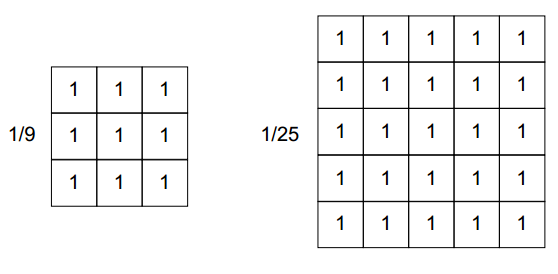
\includegraphics[width=.8\textwidth]{img/kernel-media.png}
\caption{Filtri di smoothing - Media}
\label{fig:kernel-media}
\end{figure}
\begin{figure}[!h]
\centering
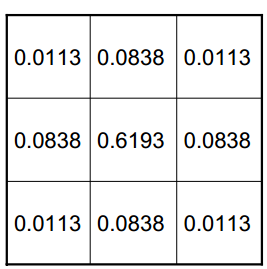
\includegraphics[width=.3\textwidth]{img/kernel-gaussiana.png}
\caption{Filtri di smoothing - Gaussiano con media 0 e dev standard 0.5}
\label{fig:kernel-gaussiana}
\end{figure}
\begin{figure}[!h]
\centering
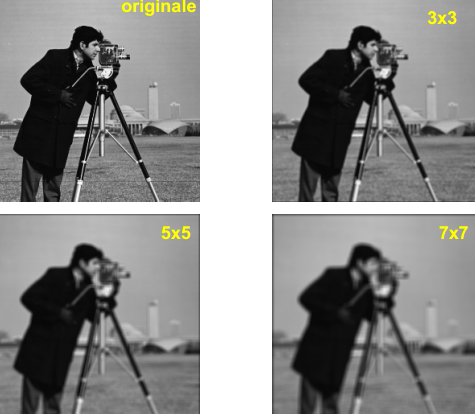
\includegraphics[width=.5\textwidth]{img/blurring.png}
\caption{Filtri di smoothing - Blurring con dimensioni maschera differenti}
\label{fig:blurring}
\end{figure}

\subsection{Filtri di sharpening}
Lo scopo di questo tipo di filtri è di incrementare la nitidezza dell’immagine 
aumentando il contrasto locale, di conseguenza, vengono enfatizzati i 
dettagli fini e le regioni di bordo, al contrario 
dei filtri di smoothing. in definitiva, tali filtri agiscono come filtri 
passa-alto rispetto alla frequenza spaziale.
I filtri di sharpening vengono realizzati tramite operazioni di 
differenziazione spaziale, l’ampiezza della risposta di un operatore 
differenziale è proporzionale al grado di discontinuità dell’immagine nel punto in cui 
l’operatore è applicato, applicare tali operatori enfatizza i 
bordi e altre discontinuità (rumore) e de-enfatizza le aree con livelli di grigio
lentamente variabili.
Nel definire un operatore differenziale del secondo  ordine, una
caratteristica da garantire è che la  risposta sia indipendente dalla
direzione della  discontinuità nell’immagine (operatore isotropo).
L’operatore derivativo isotropo più semplice è il  laplaciano:
\[
\nabla^2 = {\partial^2 \over \partial x^2_1 } + {\partial^2 \over \partial x^2_2 } + \dots = \sum_{i=1}^n \frac {\partial^2}{\partial x^2_i}
\]
L’implementazione del laplaciano per  immagini digitali si realizza
utilizzando le  implementazioni delle derivate seconde.
\begin{figure}[h]
\centering
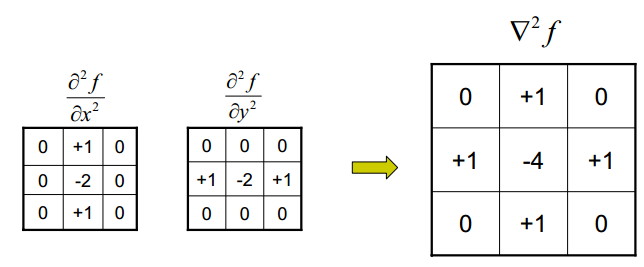
\includegraphics[width=.5\textwidth]{img/laplaciano.png}
\caption{Laplaciano}
\label{fig:laplaciano}
\end{figure}
\begin{figure}[h]
\centering
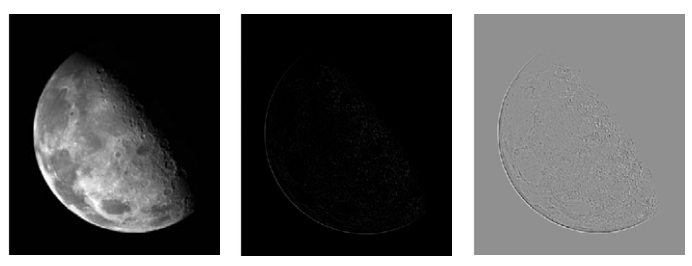
\includegraphics[width=.8\textwidth]{img/laplaciano-applicato.png}
\caption{Laplaciano applicato ad un immagine}
\label{fig:laplaciano-applicato}
\end{figure}

Il laplaciano può essere assunto come segnale correttivo da combinare con il segnale originale

\begin{figure}[h]
\centering
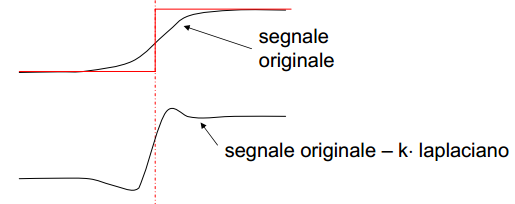
\includegraphics[width=.8\textwidth]{img/laplaciano-correttivo.png}
\caption{Correzione del segnale originale con laplaciano}
\label{fig:laplaciano-correttivo}
\end{figure}

\begin{figure}[h]
\centering
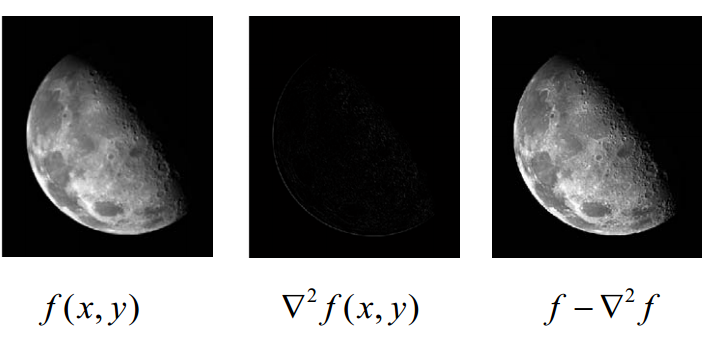
\includegraphics[width=.8\textwidth]{img/laplacian-sharpening.png}
\caption{Laplacian sharpening}
\label{fig:laplacian-sharpening}
\end{figure}

\subsection{Canny edge detector}
Nell'elaborazione di immagini, l'algoritmo di Canny è un operatore per il riconoscimento dei contorni (edge detection) ideato nel 1986 da John F. Canny. Utilizza un metodo di calcolo multi-stadio per individuare contorni di molti dei tipi normalmente presenti nelle immagini reali. Canny ha anche prodotto una teoria del riconoscimento dei contorni che si propone di spiegare i fondamenti di questa tecnica.

Per il riconoscimento dei contorni l'algoritmo di Canny usa un filtro basato sulla derivata prima di una gaussiana, e quindi i risultati prodotti sono disturbati dal rumore presente nei dati di un'immagine ``grezza'' (raw image). Per questo motivo, prima di iniziare l'elaborazione, l'immagine raw viene sottoposta a convoluzione con un filtro gaussiano. Il risultato è un'immagine con una leggera ``sfocatura'' gaussiana, in cui nessun singolo pixel è affetto da disturbi di livello significativo.

Un contorno di un'immagine può puntare verso una direzione qualsiasi, quindi l'algoritmo di Canny usa quattro filtri differenti per individuare i contorni orizzontale, verticale e diagonali dell'immagine, a cui è stato precedentemente applicato il filtro gaussiano. Per ciascun pixel risultante viene assunta come valida la direzione relativa al filtro che dà il valore maggiore. Questa direzione, combinata col valore ottenuto applicando il filtro, corrisponde a quella in cui si ha il massimo gradiente di luminosità in ciascun punto dell'immagine.

La mappa dei gradienti fornisce il valore dell'intensità luminosa in ciascun punto dell'immagine. Una forte intensità indica una forte probabilità della presenza di un contorno. Tuttavia, questa indicazione non è sufficiente a decidere se un punto corrisponde oppure no ad un contorno. Solo i punti corrispondenti a dei massimi locali sono considerati come appartenenti ad un contorno, e saranno presi in considerazione dai successivi step di elaborazione. Un massimo locale si ha nei punti in cui la derivata del gradiente si annulla.

L'estrazione dei contorni dalla mappa generata dallo step precedente si esegue con un procedimento chiamato sogliatura con isteresi. Vengono definite due soglie, una bassa ed una alta, che vengono confrontate con il gradiente in ciascun punto. Se il valore del gradiente è:
\begin{itemize}
\item inferiore alla soglia bassa, il punto è scartato;
\item superiore alla soglia alta, il punto è accettato come parte di un contorno;
\item compreso fra le due soglie, il punto è accettato solamente se contiguo ad un punto già precedentemente accettato.
\end{itemize}
La presenza di due soglie (da cui il riferimento all'isteresi) è giustificato dal fatto che è praticamente impossibile trovare un unico valore del gradiente di luminosità per discriminare se un punto appartiene o no ad un contorno. Al termine di questo step si ottiene un'immagine binaria dove ciascun pixel è marcato come appartenente o no ad un contorno. La mappa ottenuta in questo modo può essere trattata come un insieme di curve di contorno che, previa ulteriore elaborazione, può essere approssimato da una poligonale.

L'algoritmo di Canny si basa su parametri che possono influenzare sia il tempo di elaborazione che la stessa qualità dei risultati prodotti. I parametri sono:

\begin{description}
\item[Dimensione del filtro gaussiano:] il filtro sfuocatore applicato nel primo step di elaborazione influenza direttamente i risultati generati dall'algoritmo. Filtri più piccoli producono una minore sfuocatura, e permettono di riconoscere contorni più netti. Filtri più grandi producono una maggiore sfuocatura, facendo debordare i singoli pixel su aree più estese, e sono più indicati per riconoscere contorni più ampi e più sfumati - come ad esempio il contorno di un arcobaleno.
\item[Soglie applicate:] l'uso di due soglie con isteresi garantisce una maggior flessibilità rispetto alla soglia singola, ma non risolve tutti i problemi insiti nell'applicazione di un filtro di questo tipo. Una soglia settata ad un valore troppo alto può provocare la perdita di informazioni significative, mentre una soglia settata ad una valore troppo basso può far sì che informazioni irrilevanti - ad esempio semplici disturbi - possano essere interpretate come elementi importanti dell'immagine. È difficile trovare un valore generico di soglia che possa andar bene per tutte le immagini, ed in effetti non è stato ancora trovato un approccio che dia sempre risultati soddisfacenti.
\end{description}

\section{Riconoscimento di oggetti}
Object recognition (in italiano: riconoscimento di oggetti) nella computer vision è la capacità di trovare un determinato oggetto in una sequenza di immagini o video. L'uomo riconosce una moltitudine di oggetti in immagini con poco sforzo, nonostante il fatto che l'immagine degli oggetti possa variare un po' in diversi punti di vista, in diversi formati/scala o rotazione. Inoltre gli oggetti possono essere riconosciuti anche quando sono parzialmente esclusi dalla vista. Questo compito è ancora una sfida per la computer vision in generale. David Lowe (computer scientist) ha sperimentato l'estrazione e l'utilizzo di descrittori invarianti alla scala SIFT in modo da rendere il riconoscimento più affidabile.

Per ogni oggetto in un'immagine, ci sono molte ``features'', che sono caratteristiche interessanti dell'oggetto, le quali possono essere estratte in modo da fornire una descrizione ``caratteristica'' dell'oggetto. Questa descrizione estratta da una immagine campione può poi essere utilizzata per identificare l'oggetto durante il tentativo di individuare l'oggetto in una immagine di test contenente più oggetti. È importante che l'insieme di caratteristiche estratte dall'immagine campione sia insensibile a variazioni di scala delle immagini, i disturbi, l'illuminazione e distorsioni geometriche, in modo da rendere affidabile il riconoscimento.

\subsection{Template matching} 
Nel contesto dell’interpretazione delle immagini, l’obiettivo centrale è
quello di  riconoscere gli oggetti presenti all’interno di  un’immagine.
“Riconoscere” un oggetto significa verificare che nell’immagine si presente
un’istanza  dell’oggetto di cui è memorizzata una rappresentazione. Il primo e
più semplice approccio al problema  del riconoscimento nel caso delle immagini
è  quello di confrontare direttamente l’immagine  dell’oggetto cercato con
l’immagine in esame. Questo tipo di approccio si definisce template matching.
Si basa sulla misura della similarità  esistente tra il prototipo dell’oggetto
da  riconoscere (template) e (una parte dell’)  immagine. Siccome non si
conoscono a priori le regioni in cui l’istanza può presentarsi, è necessario
confrontare il template con tutte le sottoparti  dell’immagine che hanno le
stesse  dimensioni del template, a questo scopo, il template viene fatto
scorrere sequenzialmente sull’intera  immagine, valutando per ogni possibile
posizione la similarità tra il template e la  regione dell’immagine.


\begin{figure}[h]
\centering
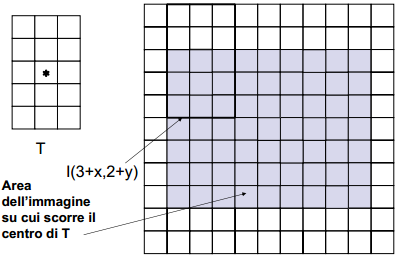
\includegraphics[width=.8\textwidth]{img/template-matching.png}
\caption{Template matching}
\label{fig:template-matching}
\end{figure}
\subsection{Funzioni per la descrizione dell'immagine}

Visti i limiti del template matching, non è 
pensabile di realizzare un sistema efficiente 
di riconoscimento che si basa sul confronto 
diretto tra le matrici di pixel.
La rappresentazione in pixel è infatti:
\begin{itemize}
\item Ridondante
\item Estremamente sensibile a modifiche anche 
insignificanti
\end{itemize}

Oltre alla matrice di pixel, esistono altri tipi di 
rappresentazione più compatte e più utili ai 
fini del riconoscimento, qlcune di queste sono basate sul contorno 
dell’oggetto:
\begin{itemize}
\item Chain code
\item Approssimazione poligonale
\item Signatures
\end{itemize}

\subsection{Signature} Una signature è una rappresentazione  monodimensionale
del contorno di un oggetto, l’idea di base è di ridurre la  rappresentazione
del contorno (tipicamente  bidimensionale) ad una funzione  monodimensionale,
presumibilmente più  facile da gestire.Un tipico esempio di signature è data
dall’andamento della distanza dei punti del contorno  dal baricentro
dell’oggetto al variare di un angolo $\theta$. Questo tipo di rappresentazione
è indipendente rispetto alla traslazione e può  essere realizzata in modo da
poter essere  poco sensibile rispetto a

\begin{description}
\item[Rotazione]Scegliendo sempre lo stesso punto di inizio (es. il 
punto del contorno più lontano dal baricentro o 
l’intersezione con l’asse principale di inerzia).
\item[Scala]Normalizzando i valori della funzione rispetto al valore 
massimo o alla deviazione standard.
\end{description}

\begin{figure}[h]
\centering
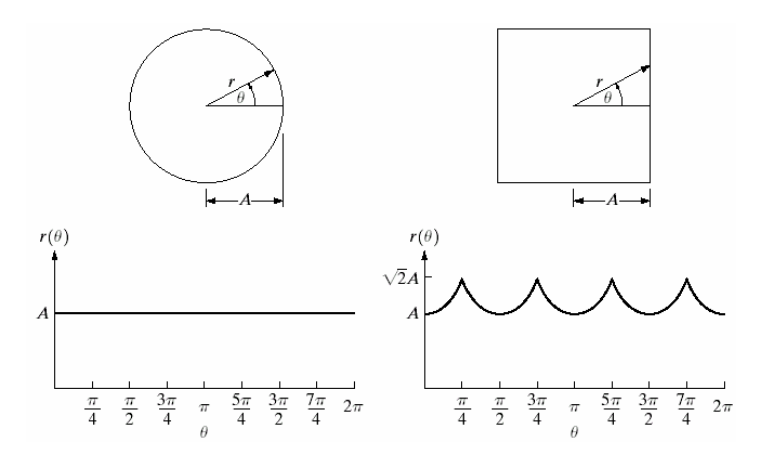
\includegraphics[width=.8\textwidth]{img/signatures.png}
\caption{Signatures}
\label{fig:signatures}
\end{figure}

\subsection{Dalla rappresentazione alla descrizione} Sebbene altri tipi di
rappresentazione siano più  efficaci rispetto alla semplice matrice di pixel,
ai  fini del riconoscimento risultano essere ancora  ridondanti e sensibili a
variazioni non  significative, è quindi opportuno considerare, invece della
rappresentazione dell’oggetto di interesse,  una sua descrizione, cioè  un
insieme di misure o di proprietà qualitative  che permettano di caratterizzare
completamente  l’oggetto ai fini del riconoscimento, siano insensibili a
variazioni non significative presenti  sulle istanze dell’oggetto e consentano
di discriminare tra istanze di oggetti  diversi

\endinput